\documentclass[11pt]{article}

\usepackage{fullpage}
\usepackage{graphicx}

\addtolength{\topmargin}{-0.6in}
\addtolength{\textheight}{1in}

\begin{document}

\title{Webapps Group Project: Project Management Report}
\author{Group 21: Kam Chiu, Ho Law, Jiranart Vacheesuthum, Vasin Wongrassamee}

\maketitle

\section{Git}
Git is used for version control, assisting distributed, non-linear workflows throughout the iterations.

Figure 1 \& 2 show major changes to the database models implemented at the start of an iteration. Then, new features that depend on the new database structures can be implemented simultaneously on separate branches. Finally, the branches are merged and minor bug fixes and optimisations are made.

Figure 3 shows separate branch of significant or fundemental changes that might break the existing system, while the existing system continues to be able to function and provide demos.

\begin{figure}[h]
\begin{minipage}{.5\textwidth}
  \centering
  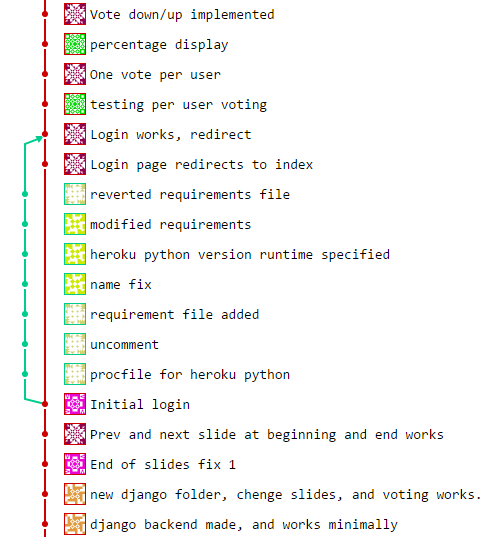
\includegraphics[width=.6\linewidth]{branch.png}
  \caption{Git commit network for iteration 1}
\end{minipage}%
\begin{minipage}{.5\textwidth}
  \centering
  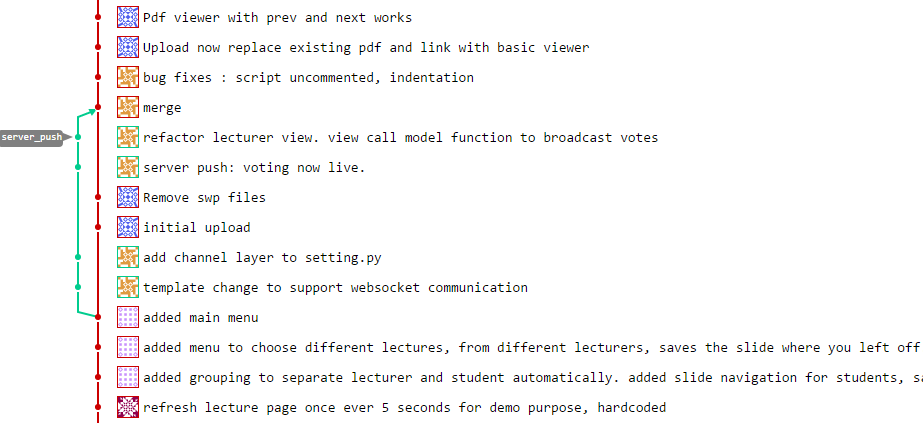
\includegraphics[width=.9\linewidth]{branch1.png}
  \caption{Git commit network for iteration 2}
\end{minipage}
\begin{minipage}{.5\textwidth}
  \centering
  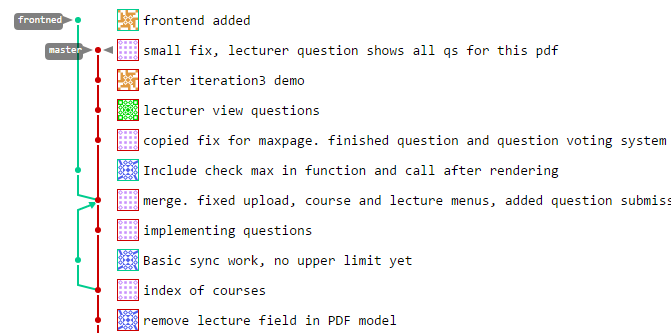
\includegraphics[width=.9\linewidth]{branch2.png}
  \caption{Git branching for experiments}
\end{minipage}%
\begin{minipage}{.5\textwidth}
  \centering
  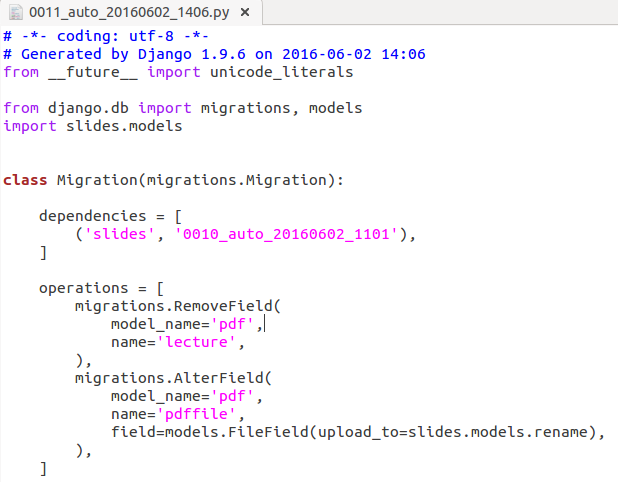
\includegraphics[width=.7\linewidth]{migration.png}
  \caption{An auto created Django migration}
\end{minipage}
\end{figure}

\section{Django Migrations}
Migrations in Django acts as version control for the database schema. Migrations are created automatically based on changes in the model.

\end{document}
